%%%%%%%%%%%%%%%%%%%%%%%%%%%%%%%%%%%%%%%%%%%%%%%%%%%%%%%%%%%%%%%%%%%%%%%%%%%%%%%%
%%  Sample document for preparing papers to  "Avtomatika i Telemekhanika"
%%  charset=utf-8
%%%%%%%%%%%%%%%%%%%%%%%%%%%%%%%%%%%%%%%%%%%%%%%%%%%%%%%%%%%%%%%%%%%%%%%%%%%%%%%%

\documentclass[12pt]{a&t}
\usepackage{graphicx}
\usepackage{bm}
\usepackage{url}
\usepackage{multirow}

\usepackage{autonum}

\begin{document}  %%%!!!

\year{2021}

\title{Байесовская дистилляция моделей глубокого обучения}%
\thanks{Настоящая статья содержит результаты проекта Математические методы интеллектуального анализа больших данных, выполняемого в рамках реализации Программы Центра компетенций Национальной технологической инициативы «Центр хранения и анализа больших данных», поддерживаемого Министерством науки и высшего образования Российской Федерации по Договору МГУ им. М.В.Ломоносова с Фондом поддержки проектов Национальной технологической инициативы от 11.12.2018 № 13/1251/2018. Работа выполнена при поддержке РФФИ (проекты 19-07-01155, 19-07-00875).}

\authors{А.В.~ГРАБОВОЙ\\
(Московский физико-технический институт, Москва)\\
В.В.~СТРИЖОВ, д-р~физ-мат.~наук\\
(Вычислительный центр имени А.\,А. Дородницына ФИЦ ИУ РАН)}

\maketitle

\begin{abstract}
Исследуется проблема понижения сложности аппроксимирующих моделей. 
Рассматриваются методы, основанные на дистилляции моделей глубокого обучения. 
Вводятся понятия учителя и ученика. Предполагается, что модель ученика имеет меньшее число параметров, чем модель учителя. 
Предлагается байесовский подход к выбору модели ученика. 
Авторами предложен метод назначения априорного распределения параметров ученика на основе апостериорного распределения параметров модели учителя. 
%Авторами предложен метод построения функции распределения априорного распределения.
Так как пространства параметров учителя и ученика не совпадают, предлагается механизм сопоставления этих пространств путем изменения структуры учителя.
Проводится теоретический анализ предложенного механизма сопоставления. Вычислительный эксперимент проводится на синтетических и реальных данных. В качестве реальных данных рассматривается выборка FashionMNIST.

\smallskip\\
\textit{Ключевые слова}: выбор модели; байесовский вывод; дистилляция модели; локальные преобразования; преобразования вероятностных пространств.
\end{abstract}

\section{Введение}
Исследуется проблема снижения числа обучаемых параметров моделей машинного обучения. Примерами таких моделей, с избыточным число параметров, являются AlexNet~\cite{Krizhevsky2012}, VGGNet~\cite{Simonyan2014}, ResNet~\cite{Kaiming2015}, BERT~\cite{Devlin2018, Vaswani2017}, mT5~\cite{Linting2021}, GPT3\cite{Brown2020} и другие.
\begin{table}[h!]
\caption{Число параметров в моделях машинного обучения.}
\label{tb:intro:1}
\begin{center}
\resizebox{\textwidth}{!}{
\begin{tabular}{|l|l|l|l|l|l|l|}
\hline
Название               & AlexNet     & VGGNet      & ResNet      & BERT     & mT5   & GPT3  \\ \hline
Год                          & 2012        & 2014        & 2015        & 2018     & 2020  & 2020  \\ \hline
Тип данных             & изображение & изображение & изображение & текст    & текст & текст \\ \hline
Число параметров, млрд & $0{,}06$    & $0{,}13$    & $0{,}06$    & $0{,}34$ & $13$  & $175$ \\ \hline
\end{tabular}
}
\end{center}
\end{table}
Табл.~\ref{tb:intro:1} описывает глубокие модели машинного обучения.
Число параметров моделей машинного обучения с годами растет.
Это влечет снижение интерпретируемости моделей.
Данная проблема рассматривается в специальном классе задач по состязательным атакам (англ. adversarial attack)~\cite{Zheng2020}.
Большое число параметров требует больших вычислительных ресурсов.
Из-за этого данные модели не могут быть использованы в мобильных устройствах.
Для снижения числа параметров предложен метод дистилляции модели~\cite{Hinton2015, Vapnik2015, Lopez2016}.
Дистиллируемая модель с большим числом параметров называется~\textit{учитель}, а модель получаемая путем дистилляции называется~\textit{ученик}.
При оптимизации параметров модели ученика используется модель учителя с фиксированными параметрами.
\begin{definition}
Дистилляция модели~--- снижение сложности модели путем выбора модели в множестве более простых моделей на основе параметров и ответов более сложной фиксированной модели.
\end{definition}

Идея дистилляции предложена в работах Дж.\,Е. Хинтона и В.\,Н. Вапником~\cite{Hinton2015, Vapnik2015, Lopez2016}. В этих работах предлагается использовать ответы учителя в качестве целевой переменной для обучения модели ученика.
Поставлен ряд экспериментов, в которых проводилась дистилляция моделей для задачи классификации машинного обучения.
Базовый эксперимент на выборке MNIST~\cite{mnist} показал применимость метода для дистилляции избыточно сложной нейросетевой модели в нейросетевую модель меньшей сложности.
Эксперимент по дистилляции ансамбля моделей в одну модель для решения задачи распознания речи. Также в работе~\cite{Hinton2015} был проведен эксперимент по обучению экспертных моделей на основе одной модели с большим числом параметров при помощи предложенного метода дистилляции на ответах учителя.

В работе~\cite{Zehao2017} предложен метод передачи селективности нейронов (англ. neuron selectivity transfer) основаный на минимизации специальной функции потерь основаной на максимальном среднем отклонении (англ. maximum mean discrepancy) между выходами всех слоев модели учителя и ученика. Вычислительный эксперимент показал эффективность данного метода для задачи классификации изображений на примере выборок CIFAR~\cite{cifar10} и ImageNet~\cite{imagenet}.

В данной работе предлагается метод,ы основанный на байесовском выводе.
В качестве априорного распределения параметров модели ученика предлагается использовать апостериорное распределение параметров модели учителя.
Решается задача сопоставления пространства параметров модели учителя и модели ученика.
Авторы предлагают подход, основаный на последовательном сопоставлении пространств параметров модели ученика и учителя. 
\begin{definition}
\label{def:structure}
Структура модели~--- множество структурных параметров модели, которые задают вид суперпозиции.
\end{definition}
\begin{definition}
\label{def:sopos}
Сопоставление параметрических моделей~--- изменение структуры модели (одной или нескольких моделей) в результате которого векторы параметров различных моделей лежат в одном пространстве.
\end{definition}
В результате сопоставления, параметры модели учителя и модели ученика лежат в одном пространстве.
Как следствие, в качестве априорного распределения параметров модели ученика выбирается апостериорное распределение параметров модели учителя.
В данной работе в качестве параметрических моделей рассматривается полносвязная нейронная сеть.
В качестве структурных параметров модели выбраны число слоев, а также размер каждого скрытого слоя.

В рамках предложенного метода сопоставления параметрических моделей не оговорен выбор порядка на множестве параметров модели учителя.
Для этого предлагается упорядочивать параметры модели учителя на основе их значимости.
Первый нейрон является наиболее значимым, а последний нейрон наименее значимым.
Порядок задается на основе отношения плотности распределения упорядочивваемого параметра к плотности распределения параметра в нуле~\cite{graves2011} или на основе метода Белсли~\cite{grabovoy2019}.
В рамках данной работы порядок на параметрах в рамках одного слоя задается случайный образом.

В рамках вычислительного эксперимента проводится теоретический анализ. Предложенный метод дистилляции анализируется на примере синтетической выборки, а также на реальной выборке FashionMnist~\cite{fashionmnist}.

\section{Постановка задачи дистилляции}
Задана выборка
\begin{gather}
\label{eq:st:1}
\begin{aligned}
\mathfrak{D} = \left\{\left(\mathbf{x}_i, y_i\right)\right\}_{i=1}^{m}, \qquad \mathbf{x}_i \in \mathbb{R}^{n}, \quad y_i \in \mathbb{Y},
\end{aligned}
\end{gather}
где~$\mathbf{x}_i, y_i$~--- признаковое описание и целевая переменная~$i$-го объекта, число объектов в обучающей выборке обозначается~$m$. Размер признакового описания объектов обозначается~$n$. Множество~$\mathbb{Y}=\{1,\cdots,K\}$ для задачи классификации, где~$K$ число классов, множество $\mathbb{Y}=\mathbb{R}$ для задачи регрессии.

Задана модель учителя в виде суперпозиций линейных и нелинейных преобразований:
\begin{gather}
\label{eq:st:2}
\begin{aligned}
f = \bm{\sigma} \circ \mathbf{U}_T \bm{\sigma} \circ \mathbf{U}_{T-1}\circ \cdots  \mathbf{U}_2\bm{\sigma} \circ \mathbf{U}_1,
\end{aligned}
\end{gather}
где~$T$~--- число слоев модели учителя, $\bm{\sigma}$~--- функция активации, а $\mathbf{U}_t$ обозначает матрицу линейного преобразования. Матрицы~$\mathbf{U}$ соединяются в вектор параметров~$\mathbf{u}$ модели учителя~$f$:
\begin{gather}
\label{eq:st:2.1}
\begin{aligned}
\mathbf{u} = \text{vec}\bigr(\left[\mathbf{U}_T, \mathbf{U}_{T-1}, \cdots \mathbf{U}_1\right]\bigr),
\end{aligned}
\end{gather}
где~$\text{vec}$ операция векторизации соединенных матриц.
Каждая матрица~$\mathbf{U}_t$ имеет размер~$n_t\times n_{t-1},$ где $n_0=n,$ а  $n_T={1}$ для задачи регрессии и $n_T=K$ для задачи классификации на $K$ классов. Число параметров~$N_{\text{tr}}$ учителя~$f$
\begin{gather}
\label{eq:st:2.2}
\begin{aligned}
N_{\text{tr}} = \sum_{t=1}^{T}n_tn_{t-1}.
\end{aligned}
\end{gather}
Для построения вектора параметров~$\mathbf{u}$ задается полный порядок на элементов матриц~$\mathbf{U}_t$. Для полносвязнной нейронной сети вводится естественный порядок, индуцированный номером слоя~$t$, номером нейрона, и номером элемента вектора параметров нейрона: выбирается матрица~$\mathbf{U}_t$, строка этой матрицы и элемент строки.

Например, для модели учителя в задаче регрессии:
\begin{gather}
\label{eq:st:3}
\begin{aligned}
f\bigr(\mathbf{x}\bigr) = \bm{\sigma} \circ \mathbf{U}_3 \bm{\sigma} \circ \mathbf{U}_2\bm{\sigma}\circ \mathbf{U}_1\mathbf{x},
\end{aligned}
\end{gather}
вектор параметров~$\mathbf{u}$ принимает ви
\begin{gather}
\label{eq:st:4}
\begin{aligned}
\mathbf{u} = \bigr[u_1^{1,1}, \cdots, u_1^{1,n},
                                               \cdots, 
                             u_1^{n_1,1}, \cdots, u_1^{n_1,n},  
                             u_2^{1, 1}, \cdots, u_2^{1, n_1}, 
                                                \cdots, 
                            u_2^{n_2, 1}, \cdots, u_2^{n_2, n_1},
                            u_3^{1, 1}, \cdots, u_3^{1, n_2}\bigr].
\end{aligned}
\end{gather}
Пусть для вектора параметров учителя~$f$ известно апостериорное распределение параметров~$p\bigr(\mathbf{u}|\mathfrak{D}\bigr)$. 
На основе выборки~$\mathfrak{D}$ и апостериорного распределения параметров учителя~$f$ требуется выбрать модель ученика из параметрического семейства функций:
\begin{gather}
\label{eq:st:5}
\begin{aligned}
g = \bm{\sigma} \circ \mathbf{W}_L\bm{\sigma}  \circ \cdots \circ \mathbf{W}_1, \quad \mathbf{W}_l \in \mathbb{R}^{n_l \times n_{l-1}},
\end{aligned}
\end{gather}
где~$L$ число слоев модели ученика.
Число параметров~$N_{\text{st}}$ модели ученика~$g$ вычисляется аналогично выражению~\eqref{eq:st:2.2}.
Вектор параметров модели ученика~$\mathbf{w}$ строится аналогичным образом~\eqref{eq:st:2.1}.
Модель~$g$ задается своим вектором параметров~$\mathbf{w}$.
Следовательно, задача выбора модели~$g$ эквивалентна задаче оптимизации вектора параметров~$\mathbf{w}\in\mathbb{R}^{N_{\text{st}}}$.

Параметры~$\hat{\mathbf{w}} \in \mathbb{R}^{N_{\text{st}}}$ оптимизируются при помощи вариационного вывода на основе совместного правдоподобия модели и данных:
\begin{gather}
\label{eq:st:6}
\begin{aligned}
\mathcal{L}\bigr(\mathfrak{D}, \mathbf{A}\bigr) = \log p\bigr(\mathfrak{D}|\mathbf{A}\bigr) = \log \int_{\mathbf{w} \in \mathbb{R}^{N_{\text{st}}}}p\bigr(\mathfrak{D}|\mathbf{w}\bigr)p\bigr(\mathbf{w}|\mathbf{A}\bigr)d\mathbf{w},
\end{aligned}
\end{gather}
где~$p\bigr(\mathbf{w}| \mathbf{A}\bigr)$~--- априорное распределение вектора параметров модели ученика.
Так как взятие интеграла~\eqref{eq:st:6} является вычислительно сложной задачей, используется вариационный подход~\cite{graves2011, grabovoy2019}. Для этого задается вариационное распределение параметров модели ученика~$q\bigr(\mathbf{w}|\bm{\mu}, \bm{\Sigma}\bigr),$ которое аппроксимирует неизвестное апостериорное распределение~$p\bigr(\mathbf{w}|\mathfrak{D}\bigr)$
\begin{gather}
\label{eq:st:new:1}
\begin{aligned}
q\bigr(\mathbf{w}|\bm{\mu}, \bm{\Sigma}\bigr) \approx  p\bigr(\mathbf{w}|\mathfrak{D}\bigr).
\end{aligned}
\end{gather}
Далее распределение $q\bigr(\mathbf{w}|\bm{\mu}, \bm{\Sigma}\bigr)$ обозначается просто~$q\bigr(\mathbf{w}\bigr).$ Оптимизация параметров~$\mathbf{w}$ сводится к решению  задачи:
\begin{gather}
\label{eq:st:7}
\begin{aligned}
\hat{\mathbf{w}} = \arg \min_{\bm{\mu}, \bm{\Sigma}, \mathbf{w}} \text{D}_{\text{KL}}\bigr(q\bigr(\mathbf{w}|\bm{\mu}, \bm{\Sigma}\bigr)||p\bigr(\mathbf{w}|\mathbf{A}\bigr)\bigr) - \log p\bigr(\mathbf{y}|\mathbf{X}, \mathbf{w}\bigr).
\end{aligned}
\end{gather}
Выражение~\eqref{eq:st:7} не учитывает параметры учителя~$f$. Для использования информации о распределении параметов учителя предлагается рассмотреть параметры априорного распределения~$p\bigr(\mathbf{w}|\mathbf{A}\bigr)$ как функцию от апостериорного распределения учителя~$p\bigr(\mathbf{u}|\mathfrak{D}\bigr)$.

\section{Построение априорного распределения ученика}
Апостериорное распределение параметров модели учителя предполагается нормальным:
\begin{gather}
\label{eq:ap:1}
\begin{aligned}
p\bigr(\mathbf{u}|\mathfrak{D}\bigr) = \mathcal{N}\bigr(\mathbf{m}, \bm{\Sigma}\bigr),
\end{aligned}
\end{gather}
где~$\mathbf{m}$ и~$\bm{\Sigma}$ параметры этого распределения. На основе параметров~$\mathbf{m}$ и~$\bm{\Sigma}$ требуется задать параметры~$\mathbf{A}$ априорного распределения~$p\bigr(\mathbf{w}|\mathbf{A}\bigr).$
В случае, когда структура моделей учителя и ученика задаются числом слоев и размером этих слоев, то возможны следующие варианты: 1) число слоев и размер каждого слоя совпадает; 2) число слоев совпадает, а размеры различаются; 3) не совпадает число слоев.

\subsection{Учитель и ученик принадлежат одному семейству}
\label{section:one:space}
Рассмотрим следующие условия:
\begin{enumlist}
    \item число слоев модели учителя равняется числу слоев модели ученика $L=T$;
    \item размеры соответствующих слоев совпадают, другими словами, для всех $t, l$ таких, что $t=l$ выполняется $n_l = n_t,$ где $n_t$ обозначает размер $t$-го слоя учителя, а $n_l$ размер $l$-го слоя ученика.
\end{enumlist}
В случае выполнения этих условий, априорное распределение параметров модели ученика приравнивается к апостериорному распределения параметров учителя $p\bigr(\mathbf{w}|\mathbf{A}\bigr) = p\bigr(\mathbf{u}|\mathfrak{D}\bigr)$.

\subsection{Удаление нейрона в слое учителя}
Проведем согласование модели учителя и модели ученика, согласно определению~\ref{def:sopos} при помощи последовательных преобразований параметров~$\mathbf{u}$. Рассмотрим преобразование:
\begin{gather}
\label{eq:ap:2}
\begin{aligned}
\phi\bigr(t, \mathbf{u}\bigr) : \mathbb{R}^{N_{\text{tr}}} \to \mathbb{R}^{N_{\text{tr}}-2n_t}
\end{aligned}
\end{gather}
вектора~$\mathbf{u},$ которое описывает удаление одного нейрона из~$t$-го слоя учителя.
%Другими словами, преобразование~$\phi\bigr(t\bigr)$ зануляет одну из строк матрицы~$\mathbf{U}_t$. Заметим, что данное зануление влечет зануление соответствующего столбца матрицы~$\mathbf{U}_{t+1}$.
Обозначим новый вектор параметров~$\bm{\upsilon} =  \phi\bigr(t, \mathbf{u}\bigr),$ а элементы вектора, которые были удалены как~$\bar{\bm{\upsilon}}.$ Заметим, что векторы~$\bm{\upsilon}$ и $\bar{\bm{\upsilon}}$ являются случайными величинами. 
%Введем следующие обозначения:
%\begin{gather}
%\label{eq:ap:def:1}
%\begin{aligned}
%\bm{\upsilon} _{0} = \mathsf{E}\bm{\upsilon} , \quad \bar{\bm{\upsilon}}_0 = \mathsf{E}\bar{\bm{\upsilon}}, \quad  \bm{\Sigma}_{\bm{\upsilon},\bm{\upsilon}} = \text{cov}\bigr(\bm{\upsilon},\bm{\upsilon}\bigr), \quad  \bm{\Sigma}_{\bm{\upsilon},\bar{\bm{\upsilon}}} = \text{cov}\bigr(\bm{\upsilon},\bar{\bm{\upsilon}}\bigr), \quad  \bm{\Sigma}_{\bar{\bm{\upsilon}},\bar{\bm{\upsilon}}} = \text{cov}\bigr(\bar{\bm{\upsilon}},\bar{\bm{\upsilon}}\bigr),\\
%\end{aligned}
%\end{gather}
%где~$ \text{cov}\bigr(\bm{\upsilon},\bm{\upsilon}\bigr)$ обозначает ковариационную матрицу.
\begin{theorem}
\label{theorem:ap:neural}
Пусть выполняются следующие условия:
\begin{enumlist}
\item апостериорное распределение~$p\bigr(\mathbf{u}|\mathfrak{D}\bigr)$ параметров модели учителя является нормальным распределением~\eqref{eq:ap:1};
\item число слоев модели учителя равняется числу слоев модели ученика $T=L$;
\item размеры соответствующих слоев не совпадают, другими словами, для всех $t, l$ таких, что $t=l$ выполняется $n_t \leq n_l,$.
\end{enumlist}
Тогда апостериорное распределения параметров модели учителя~$p\bigr(\bm{\upsilon}|\mathfrak{D}\bigr)$ также является нормальным распределением.
%\begin{gather}
%\label{eq:ap:3}
%\begin{aligned}
%p\bigr(\bm{\upsilon}|\mathfrak{D}\bigr) = \mathcal{N}\bigr(\bm{\upsilon}_{0}+\bm{\Sigma}_{\bm{\upsilon},\bar{\bm{\upsilon}}}\bm{\Sigma}_{\bar{\bm{\upsilon}},\bar{\bm{\upsilon}}}^{-1}\left(\mathbf{0} - \bar{\bm{\upsilon}}\right), \bm{\Sigma}_{\bm{\upsilon},\bar{\bm{\upsilon}}}\bm{\Sigma}_{\bar{\bm{\upsilon}},\bar{\bm{\upsilon}}}^{-1}\bm{\Sigma}_{\bm{\upsilon},\bar{\bm{\upsilon}}}\bigr).
%\end{aligned}
%\end{gather}
\end{theorem}
\begin{proof}
Не уменьшая общности, пусть~$\phi\bigr(t, \mathbf{u}\bigr)$ удаляет $j$-й нейрон в $t$-м слое, что является удалением $j$-й строки матрицы $\mathbf{U}_t$. Заметим, что удаление $j$-й строки матрицы $\mathbf{U}_t$ влечет удаление $j$-й компоненты вектора $z_{t+1}$, где
\begin{gather}
\label{eq:ap:tr:neural:1}
\begin{aligned}
\mathbf{z}_{t} = \bm{\sigma} \circ \mathbf{U}_{t-1} \bm{\sigma} \circ \cdots  \mathbf{U}_2\bm{\sigma} \circ \mathbf{U}_1\mathbf{x}.
\end{aligned}
\end{gather}

Удаление $j$-й компоненты вектора $\mathbf{z}_{t+1}$ эквивалентно занулению~$j$-го столбца матрицы~$\mathbf{U}_{t+1}.$ Заметим, что тогда предсказание модели не зависит от параметров~$j$-й строки матрицы~$\mathbf{U}_t,$ а следовательно донными параметрами также можно пренебречь.

Найдем распределение вектора~$\bm{\upsilon}.$ Для поиска распределения вектора параметров после зануления~$j$-го столбца матрицы~$\mathbf{U}_{t+1}$ воспользуемся формулой условной вероятности~$p\bigr(\bar{\bm{\nu}}_1|\mathfrak{D}, \bm{\nu}_1=\mathbf{0}\bigr)$, а для удаления~$j$-й строки матрицы~$\mathbf{U}_{t}$ воспользуемся маргинализацией распределения~$p\bigr(\bar{\bm{\nu}}_1|\mathfrak{D}, \bm{\nu}_1=\mathbf{0}\bigr)$. Обозначим зануляемые параметры модели как~$\bm{\nu}_1,$ а удаляемые параметры как~$\bm{\nu}_2.$ Также обозначим все параметры, которые не были занулены как~$\bar{\bm{\nu}}_1 = [\bm{\upsilon}^{\mathsf{T}}, \bm{\nu}_2^{\mathsf{T}}].$ Итоговое распределение параметров принимает  вид:
\begin{gather}
\label{eq:ap:tr:1:1}
\begin{aligned}
p\bigr(\bm{\upsilon}|\mathfrak{D}\bigr)  = \int_{\bm{\nu}_2}p\bigr(\bar{\bm{\nu}}_1|\mathfrak{D}, \bm{\nu}_1=\mathbf{0}\bigr) d\bm{\nu}_2.
\end{aligned}
\end{gather}

Из свойств нормального распределения следует, что распределение
\begin{gather}
\label{eq:ap:tr:neural:2}
\begin{aligned}
p\bigr(\bar{\bm{\nu}}_1|\mathfrak{D}, \bm{\nu}_1=\mathbf{0}\bigr)
\end{aligned}
\end{gather}
также является нормальным распределением с параметрами $\bm{\mu}, \bm{\Xi}$:
\begin{gather}
\label{eq:ap:tr:1:1}
\begin{aligned}
\bm{\mu} &= \mathbf{m}_{\bar{\bm{\nu}}_1}+\bm{\Sigma}_{\bar{\bm{\nu}}_1,\bm{\nu}_1} \bm{\Sigma}_{\bm{\nu}_1,\bm{\nu}_1}^{-1} \left(\mathbf{0} - \mathbf{m}_{\bm{\nu}_1}\right), \\
 \bm{\Xi} &= \bm{\Sigma}_{\bar{\bm{\nu}}_1,\bar{\bm{\nu}}_1} - \bm{\Sigma}_{\bar{\bm{\nu}}_1,\bm{\nu}_1} \bm{\Sigma}_{\bm{\nu}_1,\bm{\nu}_1}^{-1} \bm{\Sigma}_{\bar{\bm{\nu}}_1,\bm{\nu}_1},
\end{aligned}
\end{gather}
где введены обозначения~$\mathbf{m}_{\bar{\bm{\nu}}_1}, \mathbf{m}_{\bm{\nu}_1}$ соответствует подвектору вектора~$\mathbf{m},$ который относится к параметрам~$\bar{\bm{\nu}}_1$ и $\bm{\nu}_1$ соответсвенно. Ковариационная матрица~$\bm{\Sigma}_{\bar{\bm{\nu}}_1,\bm{\nu}_1}$ обозначает подматрицу матрицы~$\bm{\Sigma},$ которая соответсвует ковариационной матрицей между параметрами~$\bar{\bm{\nu}}_1$ и $\bm{\nu}_1.$

Распределение~$p\bigr(\bm{\upsilon}|\mathfrak{D}\bigr)$ найдем при помощи маргинализации распределения \eqref{eq:ap:tr:neural:2} по параметрам~$\bm{\nu}_2.$ Используя свойства нормального распределения получаем распределения:
\begin{gather}
\label{eq:ap:3}
\begin{aligned}
p\bigr(\bm{\upsilon}|\mathfrak{D}\bigr) = \mathcal{N}\bigr(\bm{\mu}_{\bm{\upsilon}},  \bm{\Xi}_{\bm{\upsilon}, \bm{\upsilon}}\bigr),
\end{aligned}
\end{gather}
где~$\bm{\mu}_{\bm{\upsilon}}$ обозначает подвектор вектора~$\bm{\mu},$ который относится к параметру~$\bm{\upsilon}$, а матрица~$\bm{\Xi}_{\bm{\upsilon}, \bm{\upsilon}}$ является подматрицей матрицы~$\bm{\Xi}$, которая относится к вектору параметрамов~$\bm{\upsilon}.$
\end{proof}

Теорема~\ref{theorem:ap:neural} задает апостериорное распределение параметров~\eqref{eq:ap:3} после зануления нейронов в модели нейросети --- учителя. Заметим, что аналогичным образом можно удалить сразу подмножество нейронов в рамках одного слоя. В случае, если число нейронов отличается в нескольких слоях модели нейросети учителя, то выполняется последовательно применения отображения~$\phi\bigr(t, \mathbf{u}\bigr)$ для каждого $t$-го слоя.

\subsection{Удаление слоя учителя}
%Пусть в модели учителя требуется убрать $t$-й слой. Рассмотрим следующие условия:
%\begin{enumlist}
 %   \item соответствующие размеры слоев совпадают, $n_t=n_{t-1}$;
  %  \item функция активации удовлетворяет следующему свойству $\bm{\sigma} \circ \bm{\sigma} = \bm{\sigma}$.
%\end{enumlist}
Проведем согласование модели учителя и модели ученика, согласно определению~\ref{def:sopos} при помощи последовательных преобразований вектора параметров~$\mathbf{u}$. Рассмотрим преобразование:
\begin{gather}
\label{eq:ap:4}
\begin{aligned}
\psi\bigr(t, \mathbf{u}\bigr) : \mathbb{R}^{N_{\text{tr}}} \to \mathbb{R}^{N_{\text{tr}}-n_tn_{t-1}}
\end{aligned}
\end{gather}
вектора~$\mathbf{u}$ которое описывает удаление одного~$t$-го слоя.
Обозначим новый вектор параметров~$\bm{\upsilon} = \psi\bigr(t, \mathbf{u}\bigr),$ а элементы вектора, которые были удалены как~$\bar{\bm{\upsilon}}.$ 
%Другими словами, преобразования~$\psi\bigr(t\bigr)$ превращает матрицу~$\mathbf{U}_t$ в единичную матрицу~$\mathbf{I}$. 
%Для отображения~$\psi\bigr(t\bigr)$ введем аналогичные~\eqref{eq:ap:def:1} обозначения~$\bm{\upsilon}_{0}, \bar{\bm{\upsilon}}_0, \bm{\Sigma}_{\bm{\upsilon},\bm{\upsilon}}, \bm{\Sigma}_{\bm{\upsilon},\bar{\bm{\upsilon}}}, \bm{\Sigma}_{\bar{\bm{\upsilon}},\bar{\bm{\upsilon}}}.$

\begin{theorem}
\label{theorem:ap:layer}
Пусть выполняются следующие условия:
\begin{enumlist}
\item апостериорное распределение параметров~$p\bigr(\mathbf{u}|\mathfrak{D}\bigr)$ модели учителя является нормальным распределением~\eqref{eq:ap:1};
\item соответствующие размеры слоев совпадают, $n_t=n_{t-1},$ то есть матрица~$\mathbf{U}_t$ является квадратной;
\item функция активации удовлетворяет свойству идемпотентности $\bm{\sigma} \circ \bm{\sigma} = \bm{\sigma}$.
\end{enumlist}
Тогда апостериорное распределения также описывается нормальным распределением со следующей плотностью распределения:
\begin{gather}
\label{eq:ap:5}
\begin{aligned}
p\bigr(\bm{\upsilon}|\mathfrak{D}\bigr) = \mathcal{N}\bigr(\mathbf{m}_{\bm{\upsilon}}+\bm{\Sigma}_{\bm{\upsilon},\bar{\bm{\upsilon}}} \bm{\Sigma}_{\bar{\bm{\upsilon}},\bar{\bm{\upsilon}}}^{-1} \left(\mathbf{i} - \bar{\bm{\upsilon}}\right), \bm{\Sigma}_{\bm{\upsilon},\bm{\upsilon}} - \bm{\Sigma}_{\bm{\upsilon},\bar{\bm{\upsilon}}}\bm{\Sigma}_{\bar{\bm{\upsilon}},\bar{\bm{\upsilon}}}^{-1}\bm{\Sigma}_{\bm{\upsilon},\bar{\bm{\upsilon}}}\bigr),
\end{aligned}
\end{gather}
где вектор~$\mathbf{i}$ задается следующим образом:
\[
\mathbf{i}=[\underbrace{1, 0, \cdots, 0}_{n_t}, \underbrace{0, 1, \cdots, 0}_{n_t}, \underbrace{0, 0, 1, \cdots, 0}_{n_t}, \underbrace{0, \cdots, 1}_{n_t}]^{\mathsf{T}}.
\]
\end{theorem}
\begin{proof}
Рассмотрим структуру нейронной сети с $T$ слоями и $T+1$ слоем. Не уменьшая общности для удаления рассматривается $t$-й слой, для которого выполняются условия этой теоремы. Заметим, что если $t$-й слой нейронной сети с $T+1$ слоем приравнять к единичной матрице, то он будет эквивалентным архитектуре с $T$ слоями:
\begin{gather}
\label{eq:ap:tr:2:1}
\begin{aligned}
f &= \bm{\sigma} \circ \mathbf{U}_{T+1}\bm{\sigma} \circ \mathbf{U}_T \cdots \bm{\sigma} \circ \mathbf{U}_t\bm{\sigma} \circ \cdots  \mathbf{U}_2\bm{\sigma} \circ \mathbf{U}_1 =\\
&=  \bm{\sigma} \circ \mathbf{U}_{T+1}\bm{\sigma} \circ \mathbf{U}_T \cdots \bm{\sigma} \circ \mathbf{I}\bm{\sigma} \circ \cdots  \mathbf{U}_2\bm{\sigma} \circ \mathbf{U}_1 =\\
&=  \bm{\sigma} \circ \mathbf{U}_{T+1}\bm{\sigma} \circ \mathbf{U}_T \cdots \bm{\sigma} \circ \bm{\sigma} \circ \cdots  \mathbf{U}_2\bm{\sigma} \circ \mathbf{U}_1 =^{1}\\
&=^{1}  \bm{\sigma} \circ \mathbf{U}_{T+1}\bm{\sigma} \circ \mathbf{U}_T \cdots \bm{\sigma} \circ \cdots  \mathbf{U}_2\bm{\sigma} \circ \mathbf{U}_1.
\end{aligned}
\end{gather}
\footnotetext[1]{Выполняется в силу условия теоремы об идемпотентности функции активации.}
Получаем, что удаление~$t$-го слоя нейросети эквивалентно приравнивают матрицы параметров~$t$-го слоя к единичной матрице. Распределение параметров после приравнивая к единичной матрице вычисляется при помощи условного распределения. В силу общих свойств нормального распределения условное распределения также является нормальным распределением с параметрами~$\bm{\mu}, \bm{\Xi}:$
\begin{gather}
\label{eq:ap:tr:2:2}
\begin{aligned}
\bm{\mu} &= \mathbf{m}_{\bm{\upsilon}}+\bm{\Sigma}_{\bm{\upsilon},\bar{\bm{\upsilon}}} \bm{\Sigma}_{\bar{\bm{\upsilon}},\bar{\bm{\upsilon}}}^{-1} \left(\mathbf{i} - \bar{\bm{\upsilon}}\right), \\
\bm{\Xi} &= \bm{\Sigma}_{\bm{\upsilon},\bm{\upsilon}} - \bm{\Sigma}_{\bm{\upsilon},\bar{\bm{\upsilon}}}\bm{\Sigma}_{\bar{\bm{\upsilon}},\bar{\bm{\upsilon}}}^{-1}\bm{\Sigma}_{\bm{\upsilon},\bar{\bm{\upsilon}}}\bigr),
\end{aligned}
\end{gather}
где вектор~$\mathbf{m}_{\bm{\upsilon}}$ является подвектором вектора~$\mathbf{m}$ соответсвующий параметрам~$\bm{\upsilon},$ а матрица~$\bm{\Sigma}_{\bm{\upsilon},\bar{\bm{\upsilon}}}$ является подматрицей ковариационной матрицы~$\bm{\Sigma}$ соответсвующий векторам параметров~$\bm{\upsilon}$ и~$\bar{\bm{\upsilon}}.$
\end{proof}

Теорема~\ref{theorem:ap:layer} задает апостериорное распределение~\eqref{eq:ap:5} параметров после удаления слоя нейросети. Полученное распределение $p\bigr(\bm{\upsilon}|\mathfrak{D}\bigr) $ является оценкой апостериорного распределения модели без одного слоя.

\subsection{Выполнение последовательных преобразований}
Преобразования $\phi, \psi$ согласовывают пространства параметров учителя~$f$ и ученика~$g$. После сопоставления параметрических моделей получаем, что параметры модели учителя и модели учителя принадлежат одному семейству~\ref{section:one:space}.
%После сопоставления параметров в качестве априорного распределения параметров ученика~$p\bigr(\mathbf{w}|\mathfrak{D}\bigr)$ рассматривается полученное апостериорное распределение параметров учителя~$p\bigr(\mathbf{u}'|\mathfrak{D}\bigr)$. Получаем, следующее приближение априорного распределения:
%\begin{gather}
%\label{eq:ap:6}
%\begin{aligned}
%p_g\bigr(\mathbf{w}|\mathfrak{D}\bigr) = p_{f'}\bigr(\mathbf{w}|\mathfrak{D}\bigr),
%\end{aligned}
%\end{gather}
%где данное априорное распределение используется для поиска оптимальных параметров модели ученика~$\hat{\mathbf{w}}$ с помощью~\eqref{eq:st:7}.

\section{Вычислительный эксперимент}
Проводится вычислительный эксперимент для анализа предложенного метода дистилляции на основе апостериорного распределения параметров модели учителя.

\subsection{Синтетические данные}
Проанализируем модель на синтетической выборке. Выборка построенная следующим образом:
\begin{gather}
\label{eq:ex:1}
\begin{aligned}
\mathbf{w} &= \left[w_j: w_{j}\sim \mathcal{N}\bigr(0, 1\bigr)\right]_{n\times 1}, \quad \mathbf{X} &= \left[x_{ij}: x_{ij}\sim\mathcal{N}\bigr(0, 1\bigr)\right]_{m\times n}, \\
 \mathbf{y} &= \left[y_i: y_i \sim \mathcal{N}\bigr(\mathbf{x}_i^{\mathsf{T}}\mathbf{w}, \beta\bigr)\right]_{m \times 1},
\end{aligned}
\end{gather} 
где~$\beta=0{,}1$~--- уровень шума в данных. В эксперименте число признаков~$n=10$, для обучения и тестирования было сгенерировано~$m_{\text{train}}=900$ и~$m_{\text{test}}=124$ объекта.

В качестве модели учителя рассматривалась модель~--- многослойный перцептрон с двумя скрытыми слоями \eqref{eq:st:3}. Матрицы линейных преобразований имеют размер:
\begin{gather}
\label{eq:ex:2}
\begin{aligned}
\mathbf{U}_{1} \in \mathbb{R}^{100 \times 10}, \quad \mathbf{U}_{2} \in \mathbb{R}^{50 \times 100}, \quad \mathbf{U}_{3} \in \mathbb{R}^{1 \times 50}.
\end{aligned}
\end{gather}
В качестве функции активации была выбрана функция активации $\text{ReLu}$.
Модель учителя предварительно обучена на основе вариационного вывода \eqref{eq:st:7}, где в качестве априорного распределения параметров выбрано стандартное нормальное распределение.

В качестве модели ученика были выбраны две конфигурации. Первая конфигурация получается путем удаления нейронов в модели учителя:
\begin{gather}
\label{eq:ex:3}
\begin{aligned}
g = \bm{\sigma} \circ \mathbf{W}_3\bm{\sigma} \circ \mathbf{W}_2\bm{\sigma} \circ \mathbf{W}_1,
\end{aligned}
\end{gather}
где~$\bm{\sigma}$ является нелинейной функцией активации, а матрицы линейных преобразований имеют размер:
\begin{gather}
\label{eq:ex:4}
\begin{aligned}
\mathbf{W}_{1} \in \mathbb{R}^{10 \times 10}, \quad \mathbf{W}_{2} \in \mathbb{R}^{10 \times 10},  \quad \mathbf{W}_{3} \in \mathbb{R}^{1 \times 10}.
\end{aligned}
\end{gather}
В качестве функции активации была выбрана функция активации $\text{ReLu}$.

\begin{figure}[h!]
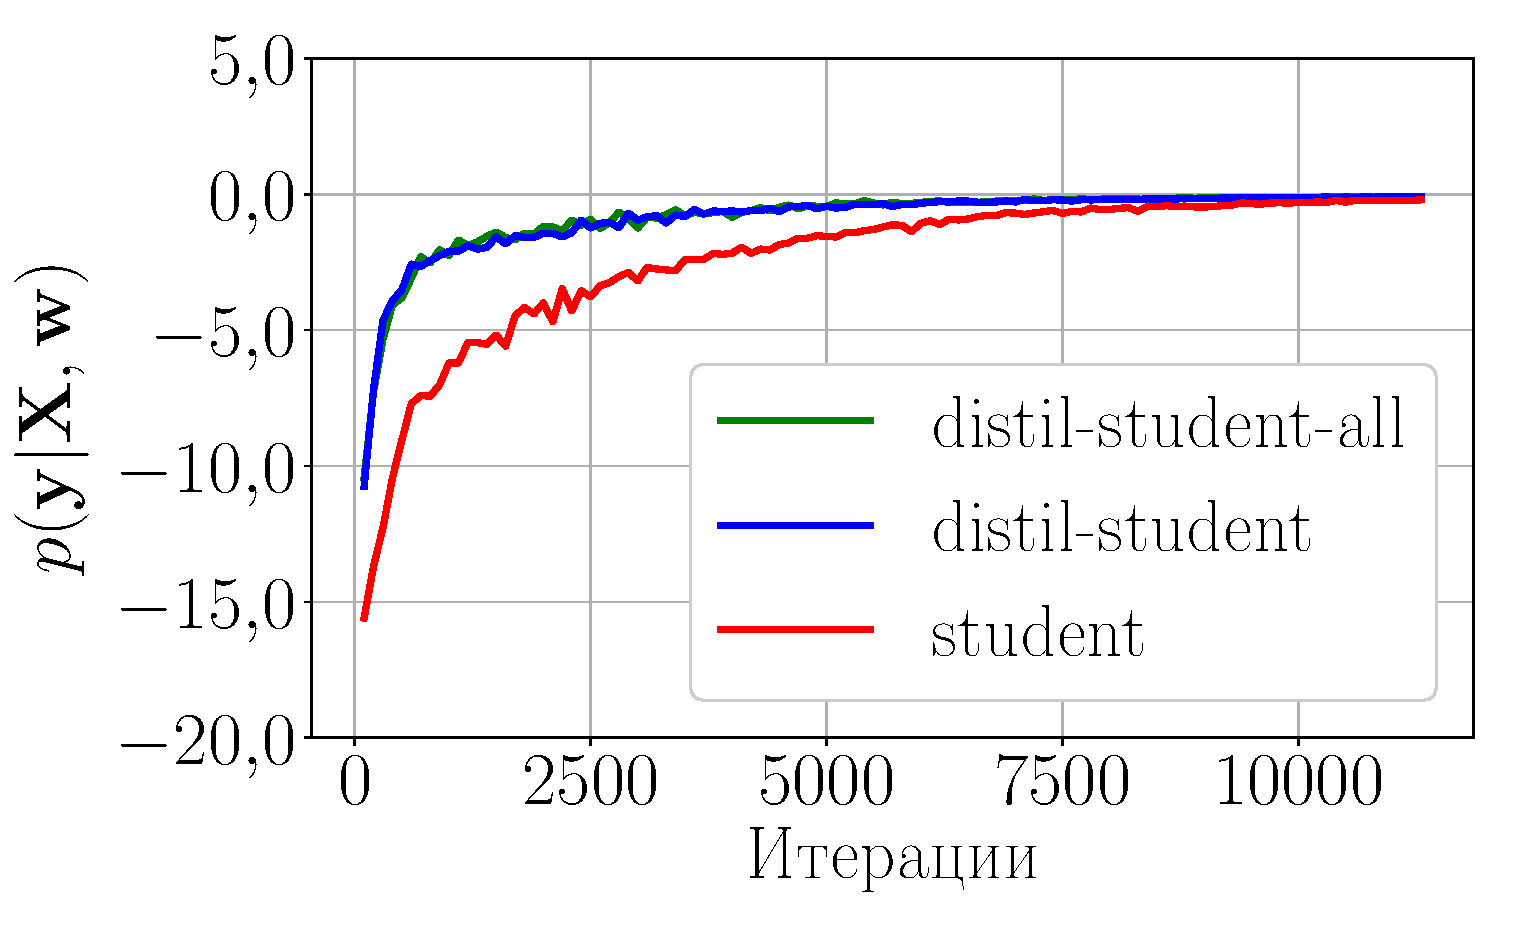
\includegraphics[width=0.5\textwidth]{synthetic_likelihood_3_layers.eps}
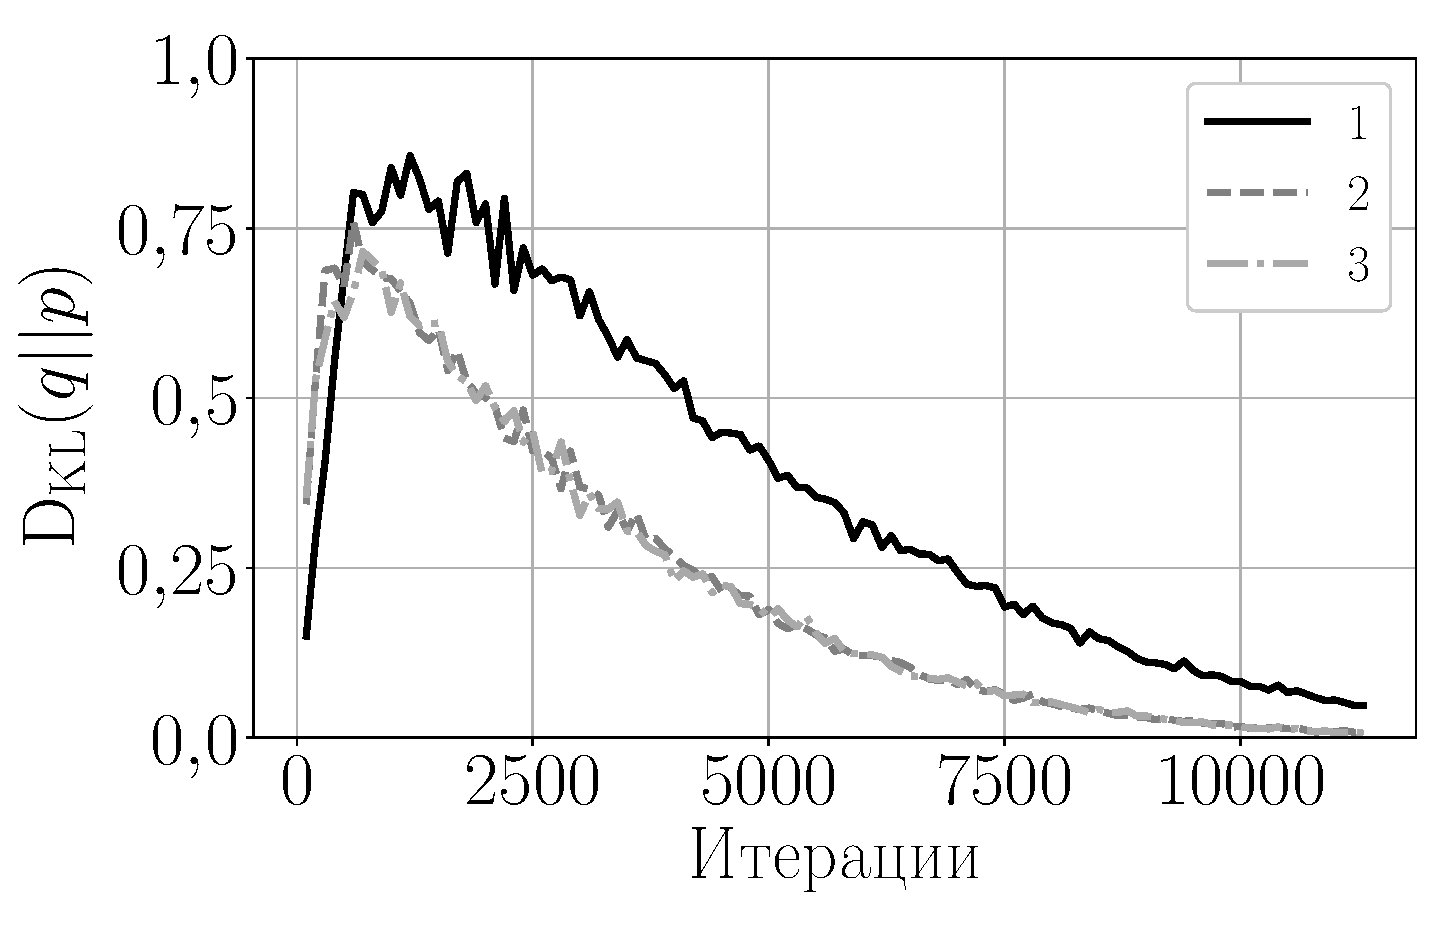
\includegraphics[width=0.5\textwidth]{synthetic_D_KL_3_layers.eps}
\caption{Структура~\eqref{eq:ex:3} модели ученика $g$. Слева: правдоподобие выборки в зависимости от номера итерации при обучении. Справа: KL--дивергенция между вариационным и априорным распределениями параметров модели.}
\label{exp:fig1}
\end{figure}

Рис.~\ref{exp:fig1} сравнивает модели ученика, со структурой~\eqref{eq:ex:3}. Представлено сравнение разных моделей: модель без дистилляции, где в качестве априорного распределения выбирается стандартное нормальное распределение (на легенде обозначается student); модель с частичной дистилляцией, где в качестве среднего значения параметров выбираются параметры согласно выражения~\eqref{eq:ap:3}, а ковариационная матрица была приравнена к единичной матрицы (на легенде обозначается distil-student); модель с полной дистилляцией согласно выражения~\eqref{eq:ap:3} (на легенде обозначается distil-student-all). Видно, что модели ученика, где в качестве априорного распределения выбраны распределения, основанные на апостериорном распределение учителя имеют большее правдоподобие, чем модель где в качестве априорного распределения выбрано стандартное нормальное. Также заметим, что использования параметра среднего из апостериорного распределения дает основной вклад при дистилляции, так как качество моделей distil-student и distil-student-all совпадает.

Вторая конфигурация получается путем удаления слоя модели учителя:
\begin{gather}
\label{eq:ex:5}
\begin{aligned}
g = \bm{\sigma} \circ \mathbf{W}_2\bm{\sigma} \circ \mathbf{W}_1,
\end{aligned}
\end{gather}
где~$\bm{\sigma}$ является нелинейной функцией активации, а матрицы линейных преобразований имеют размер:
\begin{gather}
\label{eq:ex:6}
\begin{aligned}
\mathbf{W}_{1} \in \mathbb{R}^{1 \times 50}, \quad \mathbf{W}_{2} \in \mathbb{R}^{50 \times 10}.
\end{aligned}
\end{gather}
 В качестве функции активации была выбрана функция активации $\text{ReLu}$.

\begin{figure}[h!]
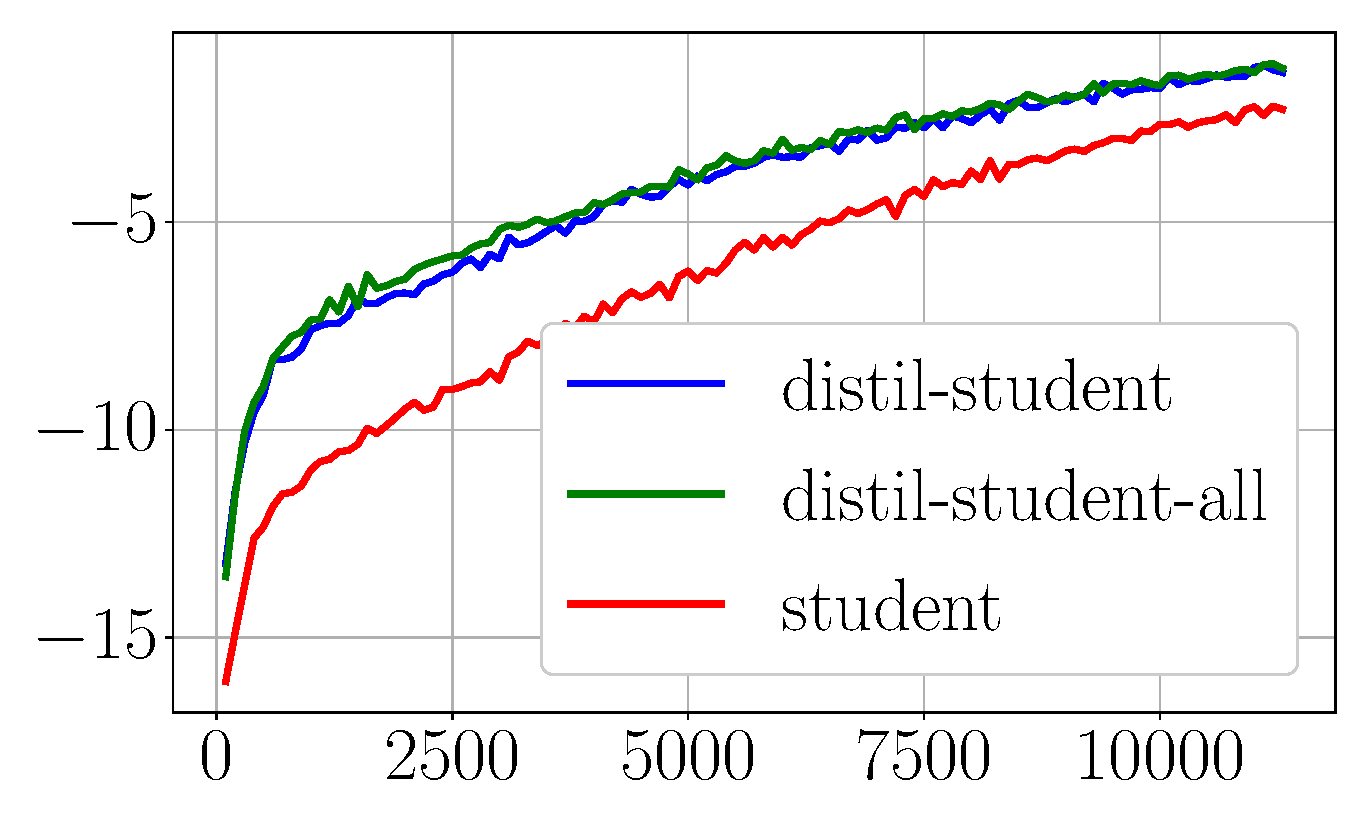
\includegraphics[width=0.5\textwidth]{synthetic_likelihood_2_layers.eps}
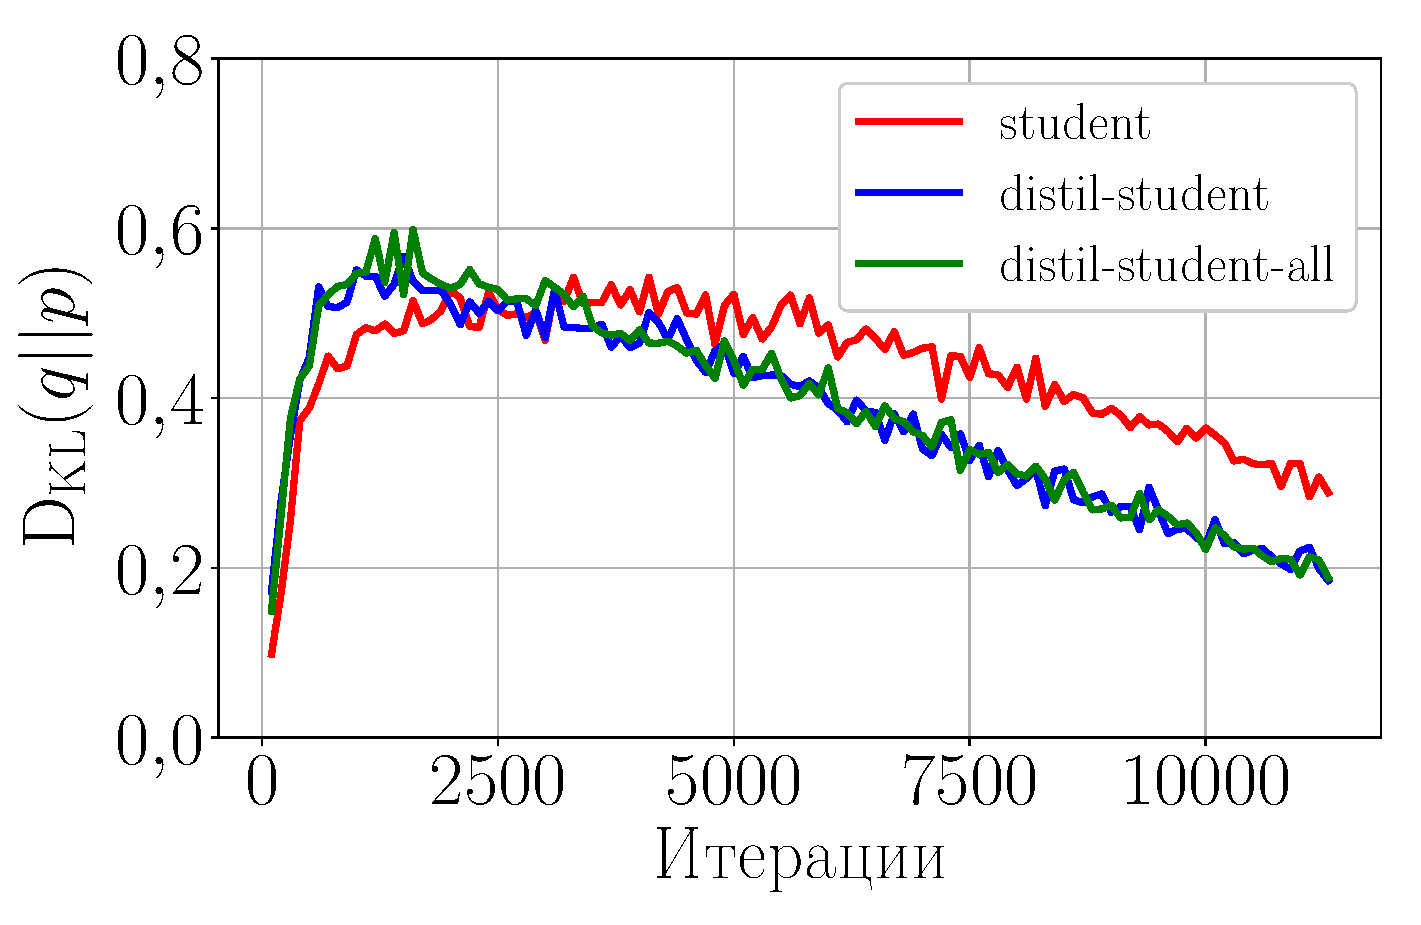
\includegraphics[width=0.5\textwidth]{synthetic_D_KL_2_layers.eps}
\caption{Структура~\eqref{eq:ex:5} модели ученика~$g$. Слева: правдоподобие выборки в зависимости от номера итерации при обучении. Справа: KL--дивергенция между вариационным и априорным распределениями параметров модели.}
\label{exp:fig2}
\end{figure}

Рис.~\ref{exp:fig2} сравнивает модели ученика со структурой~\eqref{eq:ex:5}. Аналогично рис.~\ref{exp:fig1}, на рис.~\ref{exp:fig2} представлено сравнение модели без дистилляции (student), модели с дистилляцией параметра среднего значение (distil-student) и модели с полной дистилляцией (distil-student-all). В рамках данного эксперимента, по дистилляции модели учителя в модель ученика с меньшим числом параметров получены результаты, которые подтверждают, что задание априорного распределения параметров ученика позволяет улучшить число итераций при выборе оптимальных параметров модели ученика.

\subsection{Выборка FashionMnist}

В рамках данного эксперимента проводился анализ байесовского подхода к дистилляции на реальных данных.  В качестве реальных данных выбрана выборка FashionMnist~\cite{fashionmnist} которая является задачей классификации изображений на 10 классов.

В качестве модели учителя рассматривалась модель многослойный перцептрон с двумя скрытыми слоями \eqref{eq:st:3}. Матрицы линейных преобразований имеют размер:
\begin{gather}
\label{eq:ex:7}
\begin{aligned}
\mathbf{U}_{1} \in \mathbb{R}^{800 \times 784}, \quad \mathbf{U}_{2} \in \mathbb{R}^{50 \times 800}, \quad \mathbf{U}_{3} \in \mathbb{R}^{10 \times 50},
\end{aligned}
\end{gather}
В качестве функции активации была выбрана функция активации $\text{ReLu}$.
Модель учителя предварительно обучена на основе вариационного вывода \eqref{eq:st:7}, где в качестве априорного распределения параметров выбрано стандартное нормальное распределение.

В качестве модели ученика были выбрана конфигурация с одним скрытым слоем~\eqref{eq:ex:5}, где матрицы линейных преобразований имеют размер:
\begin{gather}
\label{eq:ex:7}
\begin{aligned}
\mathbf{W}_{1} \in \mathbb{R}^{50 \times 784}, \quad \mathbf{W}_{2} \in \mathbb{R}^{50 \times 10}.
\end{aligned}
\end{gather}
В качестве функции активации была выбрана функция активации $\text{ReLu}$.

\begin{figure}[h!]
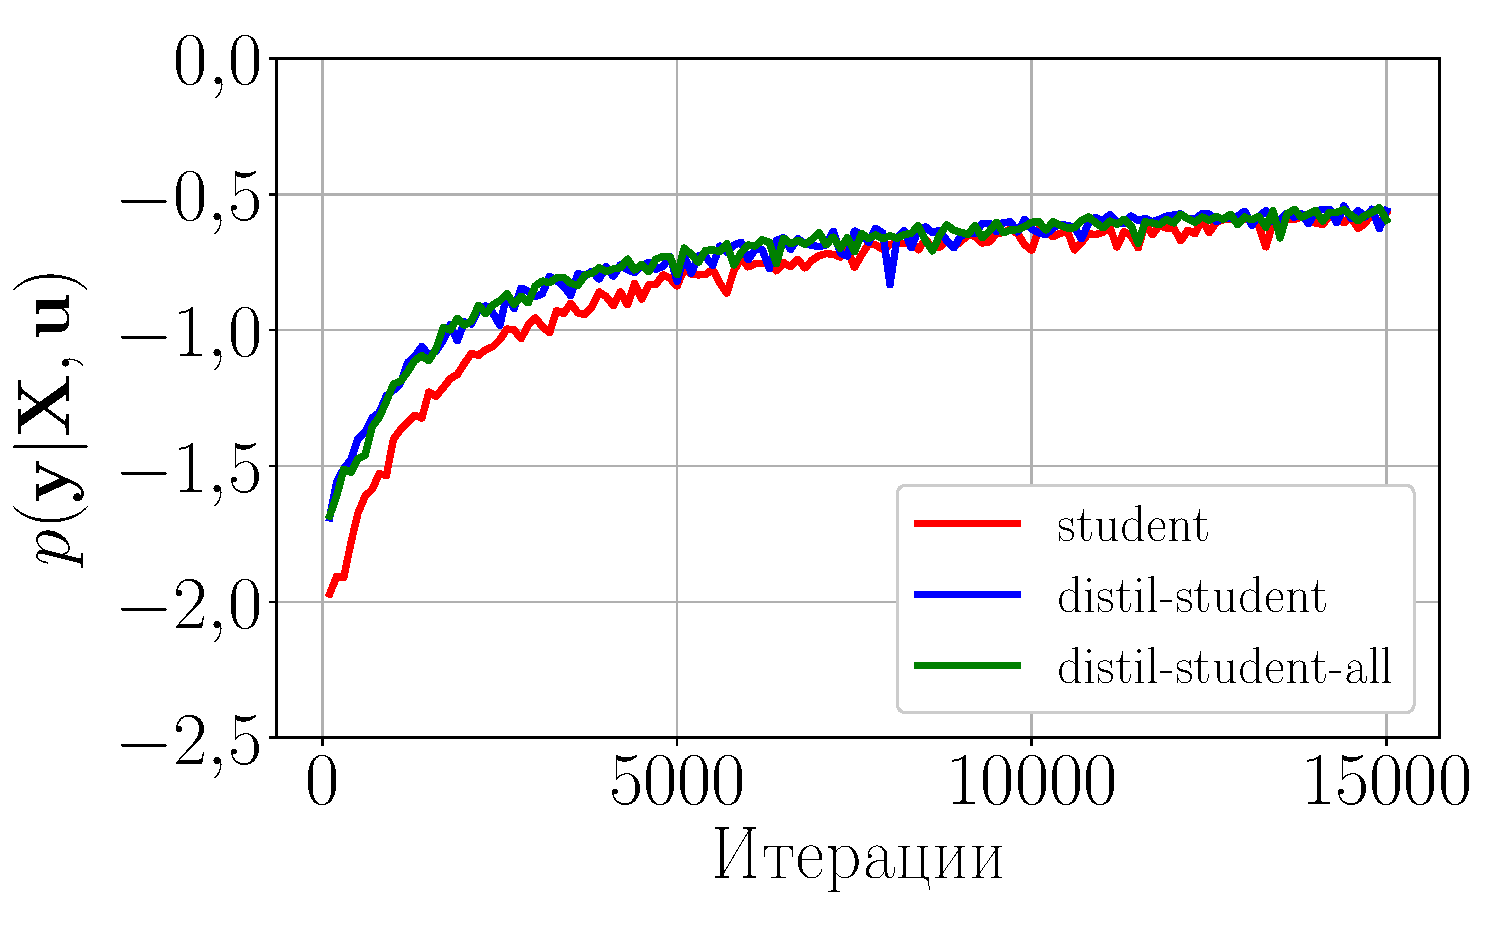
\includegraphics[width=0.5\textwidth]{fashionmnist_likelihood_2_layers.eps}
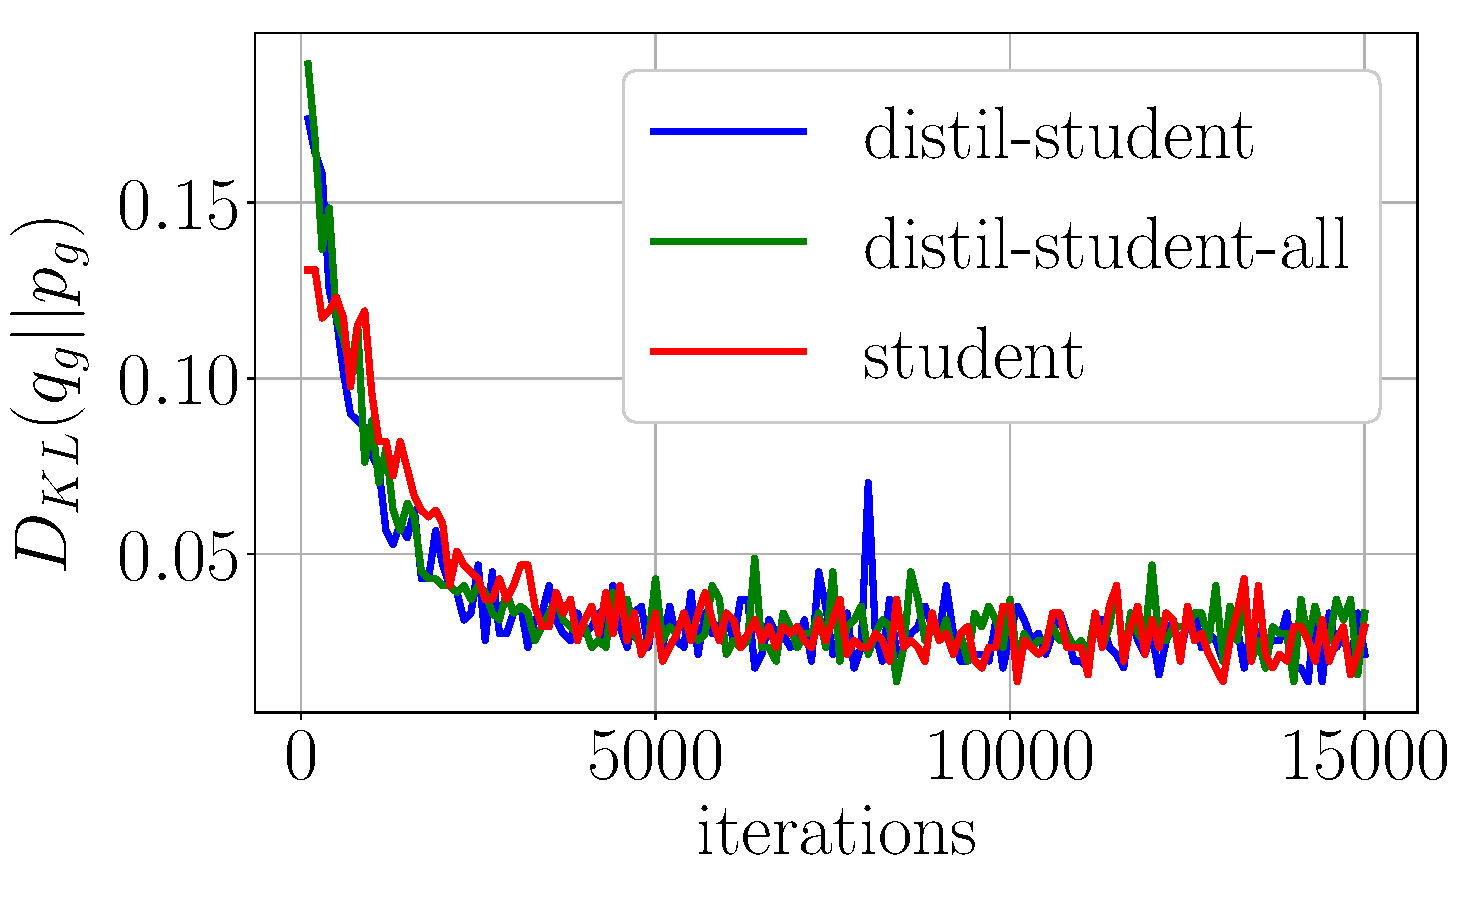
\includegraphics[width=0.5\textwidth]{fashionmnist_D_KL_2_layers.eps}
\caption{Слева: правдоподобие выборки в зависимости от номера итерации при обучении. Справа: KL--дивергенция между вариационным и априорным распределениями параметров модели.}
\label{exp:fig3}
\end{figure}

Рис.~\ref{exp:fig3} сравнивает модели ученика с разными априорными распределениями параметров.
Аналогично синтетическому эксперименту, модель, где в качестве априорного распределения использовалось стандартное нормальное распределение, сравнивалась с моделью, где параметры распределения определялись на основе формулы~\eqref{eq:ap:5}. Видно, что у моделей с заданием априорного распределения на основе апостериорного распределения параметров учителя правдоподобие выборки выше, чем у модели, где в качестве априорного распределения выбрано стандартное нормальное распределение.

\begin{table}[]
\caption{Сводная таблица результатов вычислительного эксперимента.}
\label{tb:fn:1}
\begin{center}
\begin{tabular}{|l|c|c|c|c|llll}
\cline{1-5}
                 & teacher           & student        & distil-student & distil-student-all &                           &                      &                      &                      \\ \cline{1-5}
\multicolumn{5}{|c|}{Эксперимент на синтетической выборке (удаление нейрона)}             &                      &                      &                      &                      \\ \cline{1-5}
Структура            & $[10,100,50,1]$   & $[10,10,10,1]$  & $[10,10,10,1]$ & $[10,10,10,1]$    &                      &                      &                      &                      \\ \cline{1-5}
Число параметров  & 6050                    & 210                   & 210                  & 210                      &                      &                      &                      &                      \\ \cline{1-5}
Разность площадей   &   -                         & 0                       & 16559              & 16864                  &                      &                      &                      &                      \\ \cline{1-5}
\multicolumn{5}{|c|}{Эксперимент на синтетической выборке (удаление слоя)}                    & \multicolumn{1}{c}{} & \multicolumn{1}{c}{} & \multicolumn{1}{c}{} & \multicolumn{1}{c}{} \\ \cline{1-5}
Структура            & $[10,100,50,1]$   & $[10,50,1]$       & $[10,50,1]$      & $[10,50,1]$          &                      &                      &                      &                      \\ \cline{1-5}
Число параметров    &   6050                       &          550                &          550               &             550                &                      &                      &                      &                      \\ \cline{1-5}
Разность площадей~S    &  -                          &  0                      &  23310             & 25506                  &                      &                      &                      &                      \\ \cline{1-5}
\multicolumn{5}{|c|}{Эксперимент на выборке FashionMnist}                                                     &                      &                      &                      &                      \\ \cline{1-5}
Структура           & $[784,800,50,10]$& $[784,50,10]$   & $[784,50,10]$  & $[784,50,10]$      &                      &                      &                      &                      \\ \cline{1-5}
Число параметров    &           667700                  &          39700                &         39700                &                 39700            &                      &                      &                      &                      \\ \cline{1-5}
Разность площадей~S   & -                           & 0                       &  1165               & 1145                    &                      &                      &                      &                      \\ \cline{1-5}
\end{tabular}
\end{center}
\end{table}

В табл.~\ref{tb:fn:1} представлен результат вычислительного эксперимента. Для численного сравнения качества моделей выбрана разность площадей графика $p\bigr(\mathbf{y}|\mathbf{X}, \mathbf{u}\bigr)$ между моделью student и моделями distil-student  и 
distil-student-all соответсвенно:
\begin{gather}
\label{eq:ex:8}
\begin{aligned}
S = \sum_{s} p\bigr(\mathbf{y}|\mathbf{X}, \mathbf{u}^s_{\text{s}}\bigr) - p\bigr(\mathbf{y}|\mathbf{X}, \mathbf{u}^s_{\text{ds}}\bigr),
\end{aligned}
\end{gather}
где~$\mathbf{u}^s_{\text{s}}, \mathbf{u}^s_{\text{ds}}$ обозначает параметры модели ученика и модели дистиллированного ученика после~$s$-й итерации оптимизационного процесса. Заметим, что площадь~$S$ имеет знак: чем большее положительное число, тем дистиллированная модель лучше, чем модель построенная без учителя. В случае, если площадь~$S$ принимает отрицательное значение, то значит модель без дистилляции является лучше чем модель с дистилляцией. В рамках вычислительного эксперимента видно, что площадь~$S$ под графиками принимает положительные значения, то есть модели ученика полученные при помощи дистилляции являются лучше чем модель ученика без дистилляции.

\section{Заключение}

В данной работе проанализирована байесовская дистиляция модели учителя в модель ученика на основе вариационного вывода.
В рамках данной работы дистилляция основывается на задании априорного распределения параметров модели ученика.
Априорное распределение параметров модели ученика задается на основе апостериорного распределения параметров модели учителя.
Механизм преобразования структуры модели учителя в структуру модели ученика представлен в теореме~\ref{theorem:ap:neural} и теореме~\ref{theorem:ap:layer}.

Теорема~\ref{theorem:ap:neural} описывает механизм сопоставления параметров модели учителя и ученика в случае, если число слоев совпадает, но размер слоев различается. Теорема~\ref{theorem:ap:layer} описывает механизм сопоставления параметров модели учителя и ученика в случае, если число слоев различается.

В вычислительном эксперименте сравнивается модель ученика, которая обучена без использования распределения параметров учители и модель ученика, где в качестве априорного распределения параметров выбрано апостериорное распределение параметров модели учителя после сопоставления. В табл.~\ref{tb:fn:1} показано, что модели ученика с заданиям априорного распределения параметров на основе апостериорного распределения параметров учителя сходятся быстрее, что подтверждается положительным значением метрики~\eqref{eq:ex:8}, которая введена для численного сравнения модели без дистилляции с  дистиллированной моделью.

\begin{thebibliography}{10}
\bibitem{cifar10}
	\textit{Alex Krizhevsky and Vinod Nair and Geoffrey Hinton} CIFAR-10 (Canadian Institute for Advanced Research) // \url{http://www.cs.toronto.edu/~kriz/cifar.html}
\bibitem{imagenet}
	\textit{Deng, J., Dong, W., Socher, R., Li, L.-J., Li, K., Fei-Fei, L. } Imagenet: A large-scale hierarchical image database //  IEEE conference on computer vision and pattern recognition, 2009. P. 248--255. 
	
\bibitem{Zehao2017}
	\textit{{Huang}, Zehao and {Wang}, Naiyan} Like What You Like: Knowledge Distill via Neuron Selectivity Transfer // arXiv e-prints, 2017.
\bibitem{Zheng2020}
	\textit{Kui Ren and Tianhang Zheng and Zhan Qin and Xue Liu} Adversarial Attacks and Defenses in Deep Learning // Engineering, 2020. P. 346--360.
\bibitem{Krizhevsky2012}
	\textit{Alex Krizhevsky, Ilya Sutskever, Geoffrey Hinton} ImageNet Classification with Depp Convolutional Neural Networks // NIPS, 2012.
\bibitem{Simonyan2014}
	\textit{Karen Simonyan and Andrew Zisserman} Very Deep Convolutional Networks for Large-Scale Image Recognition // NIPS, 2014.
\bibitem{Vaswani2017}
	\textit{Vaswani A., Shazeer N., Parmar N., Uszkoreit J., Jones L., Gomez A., Kaiser L., Polosukhin I.} Attention Is All You Need // In Advances in Neural Information Processing Systems. 2017. V. 5. P. 6000--6010.
\bibitem{Devlin2018}
       \textit{Devlin J., Chang M., Lee K., Toutanova K.} BERT: Pre-training of Deep Bidirectional Transformers for Language Understanding // arXiv preprinted, 2018.
\bibitem{Brown2020}
        \textit{Tom B. Brown et al} GPT3: Language Models are Few-Shot Learners // arXiv preprinted, 2020.
\bibitem{Linting2021}
        \textit{Linting Xue and Noah Constant and Adam Roberts and Mihir Kale and Rami Al-Rfou and Aditya Siddhant and Aditya Barua and Colin Raffel.} mT5: A massively multilingual pre-trained text-to-text transformer // arXiv preprinted, 2021.
\bibitem{Ziqing2020}
        \textit{Yang, Ziqing and Cui, Yiming and Chen, Zhipeng and Che, Wanxiang and Liu, Ting and Wang, Shijin and Hu, Guoping} {T}ext{B}rewer: {A}n {O}pen-{S}ource {K}nowledge {D}istillation {T}oolkit for {N}atural {L}anguage {P}rocessing // Proceedings of the 58th Annual Meeting of the Association for Computational Linguistics: System Demonstrations.  2020. P. 9--16.
\bibitem{Kaiming2015}
	\textit{He K., Zhang X., Ren S., Sun J.} Deep Residual Learning for Image Recognition // Proc. of the IEEE Conference on Computer Vision and Pattern Recognition. Las Vegas, 2016. P. 770--778.
\bibitem{bachteev2018}
	\textit{Бахтеев О.\,Ю., Стрижов В.\,В.} Выбор моделей глубокого обучения субоптимальной сложности // АиТ. 2018. № 8. С. 129--147.
\bibitem{Hinton2015}
        \textit{Hinton G., Vinyals O., Dean J.} Distilling the Knowledge in a Neural Network // NIPS Deep Learning and Representation Learning Workshop. 2015.
\bibitem{mnist}
	\textit{LeCun Y.,  Cortes C., Burges C.} The MNIST dataset of handwritten digits, 1998. \text{http://yann.lecun.com/exdb/mnist/index.html}.
\bibitem{Vapnik2015}
	\textit{Vapnik V., Izmailov R.} Learning Using Privileged Information: Similarity Control and Knowledge Transfer // Journal of Machine Learning Research. 2015. No 16. P. 2023--2049.
\bibitem{Lopez2016}
	\textit{Lopez-Paz D., Bottou L., Scholkopf B., Vapnik V.} Unifying Distillation and Privileged Information // In International Conference on Learning Representations. Puerto Rico, 2016.
\bibitem{Ivakhnenko1994}
	\textit{Madala H., Ivakhnenko A.} Inductive Learning Algorithms for Complex Systems Modeling. Boca Raton: CRC Press Inc., 1994.
\bibitem{fashionmnist}
	\textit{Xiao H., Rasul K.,Vollgraf R.} Fashion-MNIST: a Novel Image Dataset for Benchmarking Machine Learning Algorithms // arXiv preprint arXiv:1708.07747. 2017.
\bibitem{twiter2013}
	\textit{Wilson T., Kozareva Z., Nakov P., Rosenthal S., Stoyanov V., Ritter A.} {S}em{E}val-2013 Task 2: Sentiment Analysis in Twitter // Proceedings of the Seventh International Workshop on Semantic Evaluation ({S}em{E}val 2013). Atlanta, 2013. P. 312--320.
\bibitem{LeCun1989}
	\textit{LeCun Y., Boser B., Denker J., Henderson D., Howard R., Hubbard W., Jackel L.} Backpropagation Applied to Handwritten Zip Code Recognition // Neural Computation. 1989. V. 1. No 4. P. 541--551.
\bibitem{Schmidhuber1997}
	\textit{Hochreiter S., Schmidhuber J.} Long short-term memory // Neural Computation. 1997. V. 9. No 8.  P. 1735--1780.
\bibitem{kingma2014}
	\textit{Kingma D, Ba J.} Adam: A Method for Stochastic Optimization // arXiv preprint arXiv:1412.6980. 2014.
\bibitem{graves2011}
	\textit{Graves A.} Practical Variational Inference for Neural Networks // Advances in Neural Information Processing Systems, 2011. Vol. 24. P. 2348--2356.
\bibitem{grabovoy2019}
	\textit{Grabovoy A.V., Bakhteev O.Y., Strijov V.V.} Estimation of relevance for neural network parameters // Informatics and Applications, 2019. Vol.13 No 2. P. 62--70.
\bibitem{Vapnik2015}
	\textit{Vapnik V., Izmailov R.} Learning Using Privileged Information: Similarity Control and Knowledge Transfer // Journal of Machine Learning Research. 2015. No 16. P. 2023--2049.
\bibitem{Lopez2016}
	\textit{Lopez-Paz D., Bottou L., Scholkopf B., Vapnik V.} Unifying Distillation and Privileged Information // In International Conference on Learning Representations. Puerto Rico, 2016.
 \end{thebibliography}
\end{document}
